\section{Durchführung}
\label{sec:Durchführung}
\subsection{Spektrallinien des He-Spektrums}
\label{sec:Spektrallinien des He-Spektrums}
Im ersten Teil des Messprogramms werden über das Goniometer die wichtigsten Spektrallinien des He-Spektrums lokalisiert. Hierzu wird eine Helium-Lampe vor dem Gitterspektralapparat positioniert. Zu Beginn wird der Reflexionswinkel mit dem Fernrohr eingestellt. Hier zeigt sich nahezu weißes Licht, denn es ist die Zusammensetzung aller Spektralfarben der Lampe.
Der Winkel wird nun soweit verkleinert, bis durch das Okular eine schwach violette Spektrallinie zu erkennen ist. Der zu dieser Zeit eingestellte Winkel wird notiert. Der Winkel wird solange verkleinert, bis allen Spektrallinien aus Tabelle $\ref{fig:Tabelle} $ auf diese Weise ein Winkel zugeordnet worden ist.

\begin{figure}
  \centering
  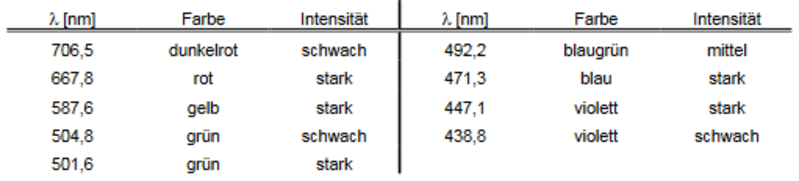
\includegraphics{ressources/Tabelle.pdf}
  \caption{Die wichtigsten sichbaren Spektrallinien des Helium-Spektrums\cite{skript}.}
  \label{fig:Tabelle}
\end{figure}

\subsection{Ausmessung der Dublettbreite bei Helium}
\label{sec:Ausmessung der Dublettbreite bei Helium}
Um den Abstand zwischen zwei Dublettlinien, bzw. die Differenz der Wellenlänge $\Delta \lambda$ zu ermitteln, reicht die Auflösung des Goniometers nicht aus.  Für die Messung wird ein Okularmikrometer verwendet. Die Differenz $\Delta s$ zwischen zwei Dublettlinien wird durch die vertikale Verschiebung des Fadenkreuzes im Okular vermessen. Zur Verschiebung wird die rechts am Fernrohr angebrachte Mikrometerschraube verwendet. Da auf der Skalentrommel der Schraube genau $100$ Teilstriche angebracht sind, wird $\Delta \lambda$ in Einheiten der Unterteilung des Okularmikrometers gemessen. Für die Umrechnung von $\Delta s$ in $\Delta\lambda$ in nm wird das Fernrohr auf zwei Spektrallinien der Helium-Lampe gerichtet, die sehr nah beieinander liegen, damit beide gleichzeitig auf dem Okular zu erkennen sind. Nun wird der Abstand $\Delta t$ ausgemessen. Aus Abbildung $\ref{fig:Winkelunterschied}$ ergeben sich die folgenden Beziehungen
\begin{align}
  \Delta s &= r \Delta \varphi
\end{align}
und
\begin{align}
  \Delta t &= r(\varphi_1 - \varphi_2) \;.
\end{align}

% Abbildung
\begin{figure}
  \centering
  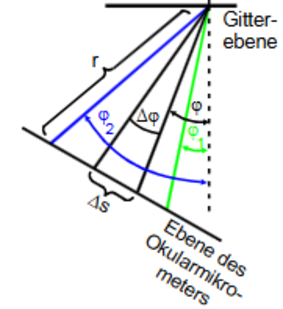
\includegraphics{ressources/delta_s.pdf}
  \caption{Ausmessung  kleiner Winkelunterschiede \cite{skript}.}
  \label{fig:Winkelunterschied}
\end{figure}

Nach weiterer Rechnung ergibt sich für die Wellenlängendifferenz
\begin{align}
  \lambda_1 - \lambda_2 = g \cos{\bar{\varphi}_\textrm{1,2}\frac{\Delta s}{r}} \qquad \qquad \text{mit} \;  \bar{\varphi}_\textrm{1,2} = \frac{1}{2}(\varphi_1 + \varphi_2)
\end{align}
In der obigen Gleichung beschreiben $\varphi_1$ und $\varphi_2$ Beugungswinkel mit den dazugehörigen Wellenlängen $\lambda_1$ und $\lambda_2$.\\
Schlussendlich ergibt sich die folgende Kalibrierungsgleichung.
\begin{align}
  \Delta \lambda &= \frac{cos{\bar{\varphi}}}{\cos{\bar{\varphi}}_\textrm{1,2}} \frac{\Delta s}{\Delta t} (\lambda_1 - \lambda_2) 
  \label{eq:deltalambda}
\end{align}


\subsection{Spektrallinien weiterer Alkalispektren}
% In diesem Teil des Messprogramm werden mit dem gleichen Verfahren aus Kapitel $\ref{sec:Spektrallinien des He-Spektrums}$ verschiedener Alkali-Metalle

In diesem Teil des Messprogramms werden weitere Spektrallinien verschiedener Alkali-Metalle mit dem  Goniometer und dem in Kapitel \ref{sec:Spektrallinien des He-Spektrums} beschriebenen Verfahren, lokalisiert.\\

Die jeweiligen Dublettlinien werden für Natrium bei rot, gelb und grüngelb, für Kalium bei gelb und grün und für Rubidium bei rot gemessen.

\subsection{Abmessung der Spektrallinien weiterer Alkalispektren}

Die zuvor lokalisierten Dubletten werden mit dem in Kapitel $\ref{sec:Ausmessung der Dublettbreite bei Helium}$ beschriebenen Verfahren präzise vermessen.









% \begin{table}
%   \centering
%   \begin{tabular}{lSSS}
%     \toprule
%     & {$ \text{Anzahl}$} & {$\text{Farbe}$}\\
%     \midrule
%     Natrium         &  1  & rot       \\
%                     &  1  & gelb      \\
%                     &  1  & gelbgruen \\
%     Kalium          &  2  & gelb      \\
%                     &  2  & gruen     \\
%     Rubidium        &  1  & rot       \\
%
%     \bottomrule
%   \end{tabular}
%   \caption{Auflistung der Abschirmkonstanten $\sigma $.}
%   \label{tab:3}
% \end{table}
